\documentclass{article}

\usepackage[heading=true]{ctex}
\usepackage[backref]{hyperref}
\usepackage{amsmath}
\usepackage{filecontents}
\usepackage{float}
\usepackage{graphicx}
\usepackage{geometry}
\usepackage{dirtree}
\usepackage{listings}
\usepackage{xcolor}
\usepackage{qtree}
\usepackage{hyperref}

\ctexset{
    section={
        number=\chinese{section},
        format+=\raggedright
    }
}
\geometry{a4paper, scale=0.7}


\title{实验二: 卷积神经网络实现}
\author{
    1190200708 熊峰\\
    \and
    1190200704 管建男\\
} 

\date{}


\begin{document}

\maketitle


\section{课题来源及研究的目的和意义}

课题的选取来自参加的信息安全竞赛中需要针对声音进行说话人识别。

通过阅读相关领域内的论文,确定了我们构建系统的方案。

本项目使用LSTM对说话人的声音的梅尔波普建立音频音频模型,
损失函数使用triplet loss\cite{schroff2015facenet}。

\section{国内外相关研究现状分析}

2018年提出的D-vector\cite{wan2018generalized}研究了
深度神经网络在小型文本相关的说话者验证任务的应用。
经过训练,网络可以在帧级别对说话人进行分类,并且对添加的噪声更加稳健。

\begin{figure}[H]
    \centering
    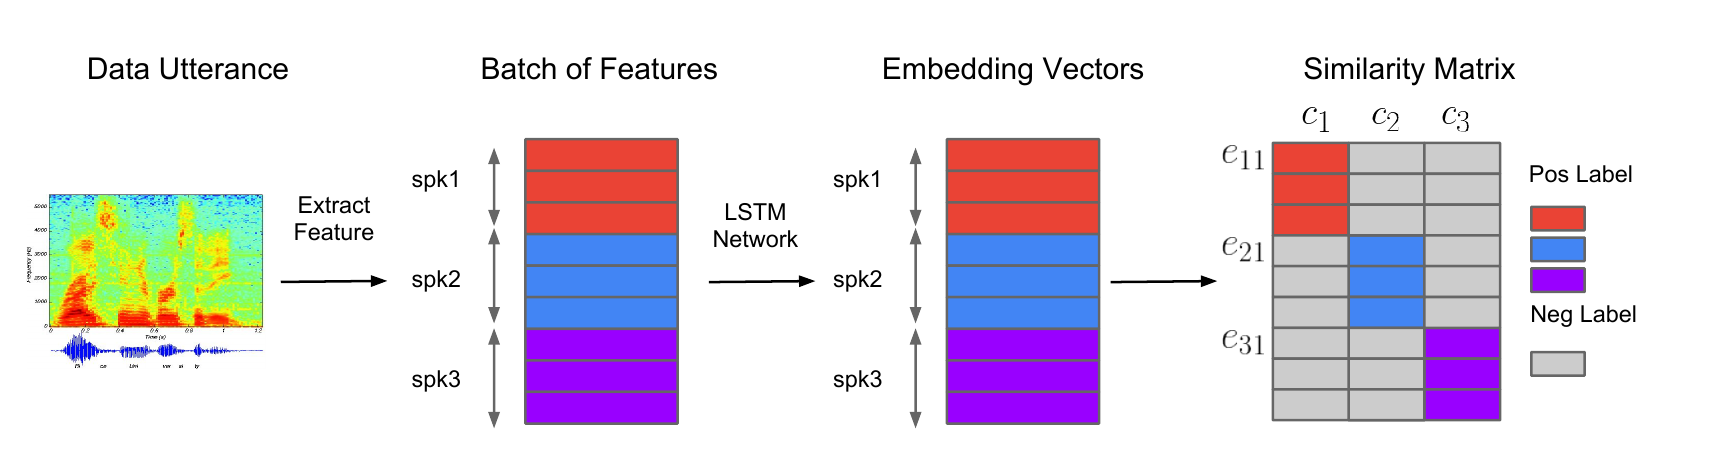
\includegraphics[width=0.8\textwidth]{figures/dvector-overview.png}
    \caption{D vector系统结构}
\end{figure}

2020年提出的Mockingjay\cite{liu2020mockingjay}是一种新的语音表示学习方法,
其中双向Transformer编码器在大量未标记的语音上进行了预训练。
以前的语音表示方法是通过对过去的帧进行条件调整并预测有关未来帧的信息来学习的。
而Mockingjay旨在通过共同调节过去和未来的环境来预测当前框架,
其大量参考了自然语言处理中的Bert模型\cite{devlin2018bert}。

\begin{figure}[H]
    \centering
    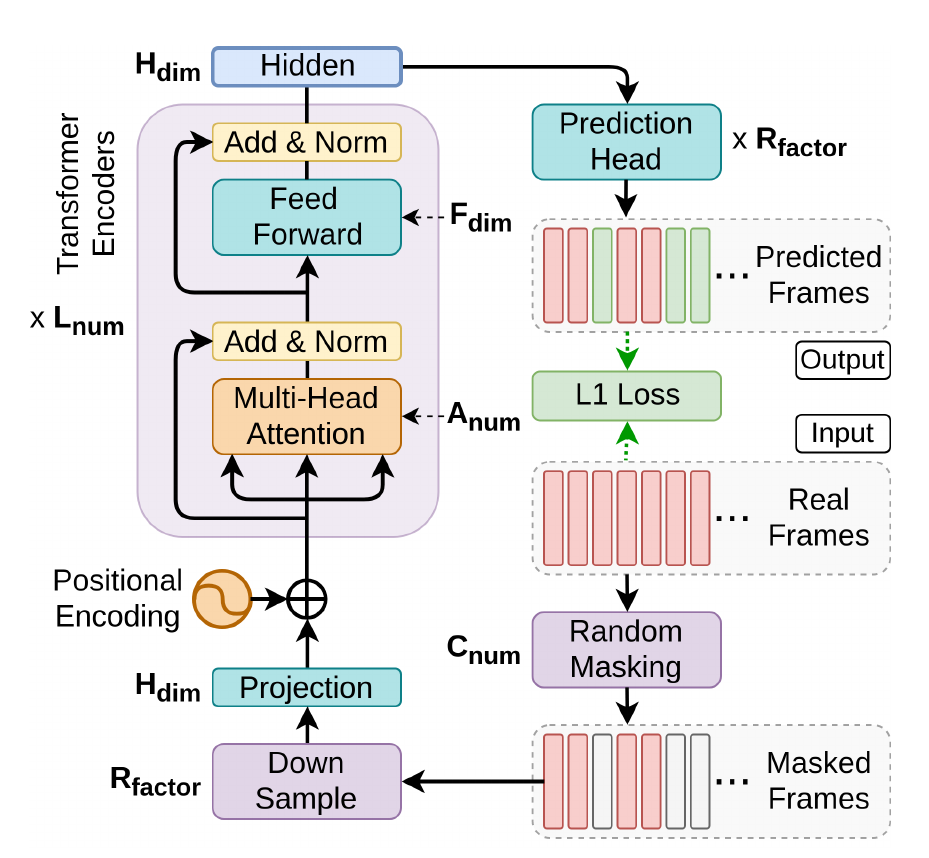
\includegraphics[width=0.6\textwidth]{figures/mockingjay-overview.png}
    \caption{Mockingjay系统结构}
\end{figure}



\section{技术方案与详细设计}

\subsection{模型设计}
长短期记忆网络是循环神经网络的一个变体,可以有效的解决简单循环神经网络的梯度爆炸或消失问题。 \par
LSTM的改进主要在以下两个方面。  \par
1. 新的内部状态\par
LSTM网络引入一个新的内部状态$c_{t}{\in}\mathcal{R}^{D}$,新的内部状态专门进行线性的循环信息传递,同时(非线性地)输出信息给隐藏层地外部状态$h_{t}{\in}\mathcal{R}^D$,内部状态$c_{t}$通过下面公式计算:\par
$$c_{t}=f_{t}{\odot}c_{t-1}+i_{t}{\odot}\widetilde{c}_{t}$$
$$h_{t}=o_{t}{\odot}tanh(c_{t})$$
其中${f_{(t)}}{\in}{[0,1]}^{D}$、$i_{t}{\in}{[0,1]}^D$、$o_{t}{\in}{[0,1]}^D$为三个门来控制信息传递的路径;$\odot$为向量元素乘积;$c_{t-1}$为上一时刻的记忆单元;$\widetilde{c}_{t}{\in}\mathcal{R}^{D}$是通过非线性函数得到的候选状态:  \par
$$\widetilde{c}_{t}=tanh(W_{c}x_{t}+U_{c}h_{t-1}+b_{c})$$
在每个时刻$t$,LSTM网络的内部状态$c_{t}$记录了到当前时刻为止的历史信息。  \par

2. 门控状态\par
LSTM网络引入门控机制来控制信息传递的路径。三个门分别为输入门$i_{t}$、遗忘门$f_{t}$和输出门$o_{t}$。这三个门的作用为  \par
遗忘门$f_{t}$控制上一个时刻的内部状态$c_{t-1}$需要遗忘多少信息;输入门$i_{t}$控制当前时刻的候选状态$\widetilde{c}_{t}$有多少信息需要保存;输出门$o_{t}$控制当前时刻的内部状态$c_{t}$有多少信息需要输出给外部状态$h_{t}$。\par

当$f_{t}=0,i_{t}=1$时,记忆单元将历史信息清空,并将候选状态向量$\widetilde{c}_{t}$写入。但此时记忆单元$c_{t}$依然和上一时刻的历史信息相关。  \par
当$f_{t}=1,i_{t}=0$时,记忆单元将复制上一时刻的内容,不写入新的信息。  \par


LSTM网络中的“门”是一种“软”门,取值在(0, 1)之间,表示以一定的比例允许信息通过.三个门的计算方式为: \par
$$i_{t}=\sigma(W_{i}x_{t}+U_{i}h_{t-1}+b_{i})$$
$$f_{t}=\sigma(W_{f}x_{t}+U_{f}h_{t-1}+b_{f})$$
$$o_{t}=\sigma(W_{o}x_{t}+U_{o}h_{t-1}+b_{o})$$
其中$\sigma(\cdot)$为Logistic函数,其输出区间为(0,1),$x_{t}$为当前时刻的输入,$h_{t-1}$为上一时刻的外部状态。  \par

\begin{figure}[H]
    \centering
    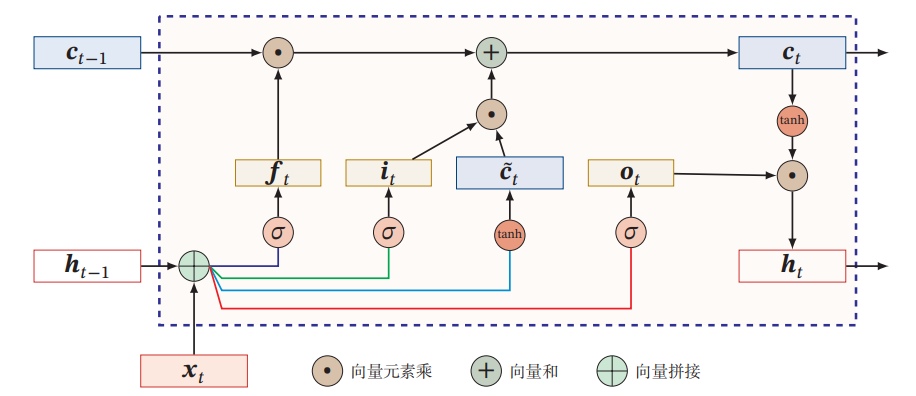
\includegraphics[width=0.6\textwidth]{figures/LSTM.png}
    \caption{LSTM网络结构}
\end{figure}


LSTM网络的循环单元结构如上图所示\cite{qiu2020nndl},其计算过程为:\par
1.首先利用上一时刻的外部状态$h_{t-1}$和当前时刻的输入$x_{t}$,计算出三个门,以及候选状态$\widetilde{c}_{t}$  \par
2.结合遗忘门$f_{t}$和输入门$i_{t}$来更新记忆单元$c_{t}$\par
3.结合输出门$o_{t}$,将内部状态的信息传递给外部状态$h_{t}$\par



通过上述LSTM循环单元,整个网络可以建立较长举例的时序依赖关系,之前的公式可以简单描述为\par

$$
    \begin{bmatrix} \widetilde{c}_{t} \\ o_{t} \\ i_{t} \\ f_{t} \end{bmatrix} = \begin{bmatrix} tanh \\ \sigma \\ \sigma \\ \sigma \end{bmatrix} \begin{pmatrix} W \begin{bmatrix} x_{t} \\ h_{t-1} \end{bmatrix} + b \end{pmatrix}
$$

$$c_{t}=f_{t}{\odot}c_{t-1}+i_{t}{\odot}{\widetilde{c}_{t}}$$

$$h_{t}=o_{t}{\odot}tanh(c_{t})$$
其中$x_{t}{\in}\mathcal{R}^{M}$为当前时刻的输入,$W{\in}\mathcal{R}^{4D{\times}(M+D)}$和$b{\in}{\mathcal{R}^{4D}}$为网络参数。  \par


\subsection{损失函数选取}
三联体损失函数,image:$x$,embedding:$f(x){\in}\mathcal{R}^{d}$,
embedding层将音频$x$转化为一个$d$维的欧式空间的向量。\par
我们想要确保一个三元组为(anchor,positive,negative)中anchor对于positive中的所有样本比negative的样本更加接近。\par
因此我们希望,$\alpha$为margin、$\mathcal{T}$为所有可能的三联体的集合,$N$为基数:  \par
$${||}f(x_{i}^{a})-f(x_{i}^{p}){||}_{2}^{2}+{\alpha}<{||}f(x_{i}^{a})-f(x_{i}^{n}){||}_{2}^{2}$$
$${\forall}(f(x_{i}^{a}),f(x_{i}^{p}),f(x_{i}^{n})){\in}\mathcal{T}$$
此时Loss为:
$$L={\sum}_{i}^{N}{[{||}f(x_{i}^{a})-f(x_{i}^{p}){||}_{2}^{2}-{||}f(x_{i}^{a})-f(x_{i}^{n}){||}_{2}^{2}+\alpha]}$$
由于部分三联体很容易满足上述要求,因此会导致网络收敛较慢,因此选择三联体非常重要。


为了确保快速收敛,关键在于违反约束的三联体。
给定$x_{i}^{a}$,我们想要选取$x_{i}^{p}$(hard positive),$argmax_{x_{i}^{p}}{||}f(x_{i}^{a})-f(x_{i}^{p}){||}_{2}^{2}$。
相似的,选取$x_{i}^{n}$(hard negative),$argmin_{x_{i}^{n}}{||}f(x_{i}^{a})-f(x_{i}^{n}){||}_{2}^{2}$.
在整个训练集上计算argmax和argmin是不可行的,一些错误的标签和糟糕的图像会导致hard positive和hard negative。

解决方法:  \par
1. 离线:每隔n步生成三联体,计算数据子集上的argmin和argmax。   \par
2. 在线:从一个小批次中选择hard positive和hard nagative示例来完成。 \par

选取hard negative的规则:
$${||}f(x_{i}^{a})-f(x_{i}^{p}){||}_{2}^{2}<{||}f(x_{i}^{a})-f(x_{i}^{n}){||}_{2}^{2}$$
这些例子被称为semi-hard,因为他们比正面的例子离anchor更远,但仍然是hard的,因为距离的平方接近于anchor的正向距离,这些负例位于边界$\alpha$内。
三元组的选择对模型训练至关重要,使用小的minibatch的SGD收敛更快,实现的时候,大一点的minibatch使用向量化计算也会加速。




\subsection{数据集选取及处理}

数据集选用openslr的\href{https://www.openslr.org/12}{LibriSpeech}语料库。
总时长约为1000小时,音频为16kHz\cite{panayotov2015librispeech}。

对于一段给定的音频,如图\ref{signal}

\begin{figure}[H]
    \centering
    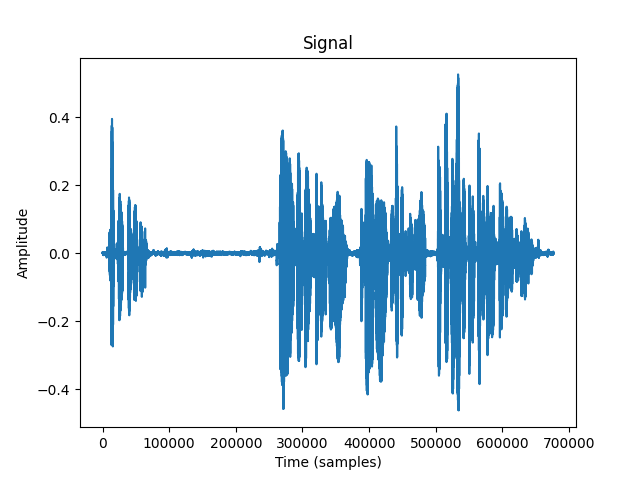
\includegraphics[width=0.6\textwidth]{figures/original-signal.png}
    \caption{音频信号}
    \label{signal}
\end{figure}

可以利用librosa库对其进行快速傅里叶变换(图\ref{fft})、提取其频谱图(图\ref{spec})、
提取其梅尔频率倒谱系数(MFCC)等操作。

\begin{figure}[H]
    \begin{minipage}[H]{0.5\linewidth}
        \centering
        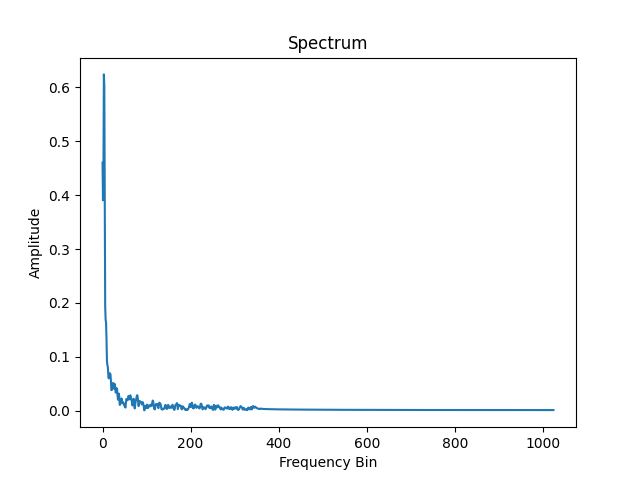
\includegraphics[width=\textwidth]{figures/fft.png}
        \caption{快速傅里叶变换}
        \label{fft}
    \end{minipage}
    \begin{minipage}[H]{0.5\linewidth}
        \centering
        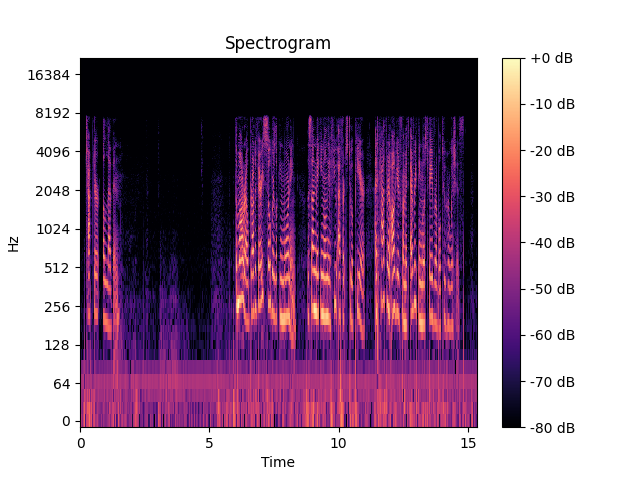
\includegraphics[width=\textwidth]{figures/spectrogram.png}
        \caption{频谱图}
        \label{spec}
    \end{minipage}
\end{figure}

本次实验中,将利用MFCC作为音频特征。对于每一段音频,将提取其180个MFCC特征。
MFCC将根据如下公式计算:

先对信号做傅立叶变换

\begin{equation}
    X[k]=FTx[n]
\end{equation}

利用此公式计算出$Y[m]$

\begin{equation}
    Y[m] = \log \left( \sum^{f_{m+1}}_{k=f_{m-1}} |X[k]|^2 B_m[k] \right)
\end{equation}

其中$B_m [k]$是梅尔频谱倒频谱的遮罩

\begin{equation}
    B_{m}[k]=\left\{
    \begin{aligned}
        0                                   & \quad k<f_{m-1} {\mbox{ or }} k>f_{m+1} \\
        {\cfrac {k-f_{m-1}}{f_{m}-f_{m-1}}} & \quad f_{m-1}\leq k\leq f_{m}           \\
        {\cfrac {f_{m+1}-k}{f_{m+1}-f_{m}}} & \quad f_{m}\leq k\leq f_{m+1}
    \end{aligned}
    \right.
\end{equation}

对$Y[m]$做反离散余弦变换(IDCT)得$c_x[n]$,因为$Y[m]$是偶函数,
故用IDCT取代反离散傅立叶变换(IDFT)\cite{cai2004hmm}。

由于每一段音频的长度互不相同,因此需要对训练数据进行重采样。
重采样遵从如下公式。

\begin{align*}
    sr_{original} & = 44100                                                            \\
    sr_{target}   & = \dfrac{sr_{original} \times 2.0833333}{duration_{sr_{original}}}
\end{align*}

其中的$2.0833333$倍缩放可以使得每一条音频都能产出一个$128 \times 180$的MFCC特征矩阵。


\section{实验分析与结论}

在开发集上的loss和acc如图\ref{dev}所示。

\begin{figure}[H]
    \begin{minipage}[H]{0.5\linewidth}
        \centering
        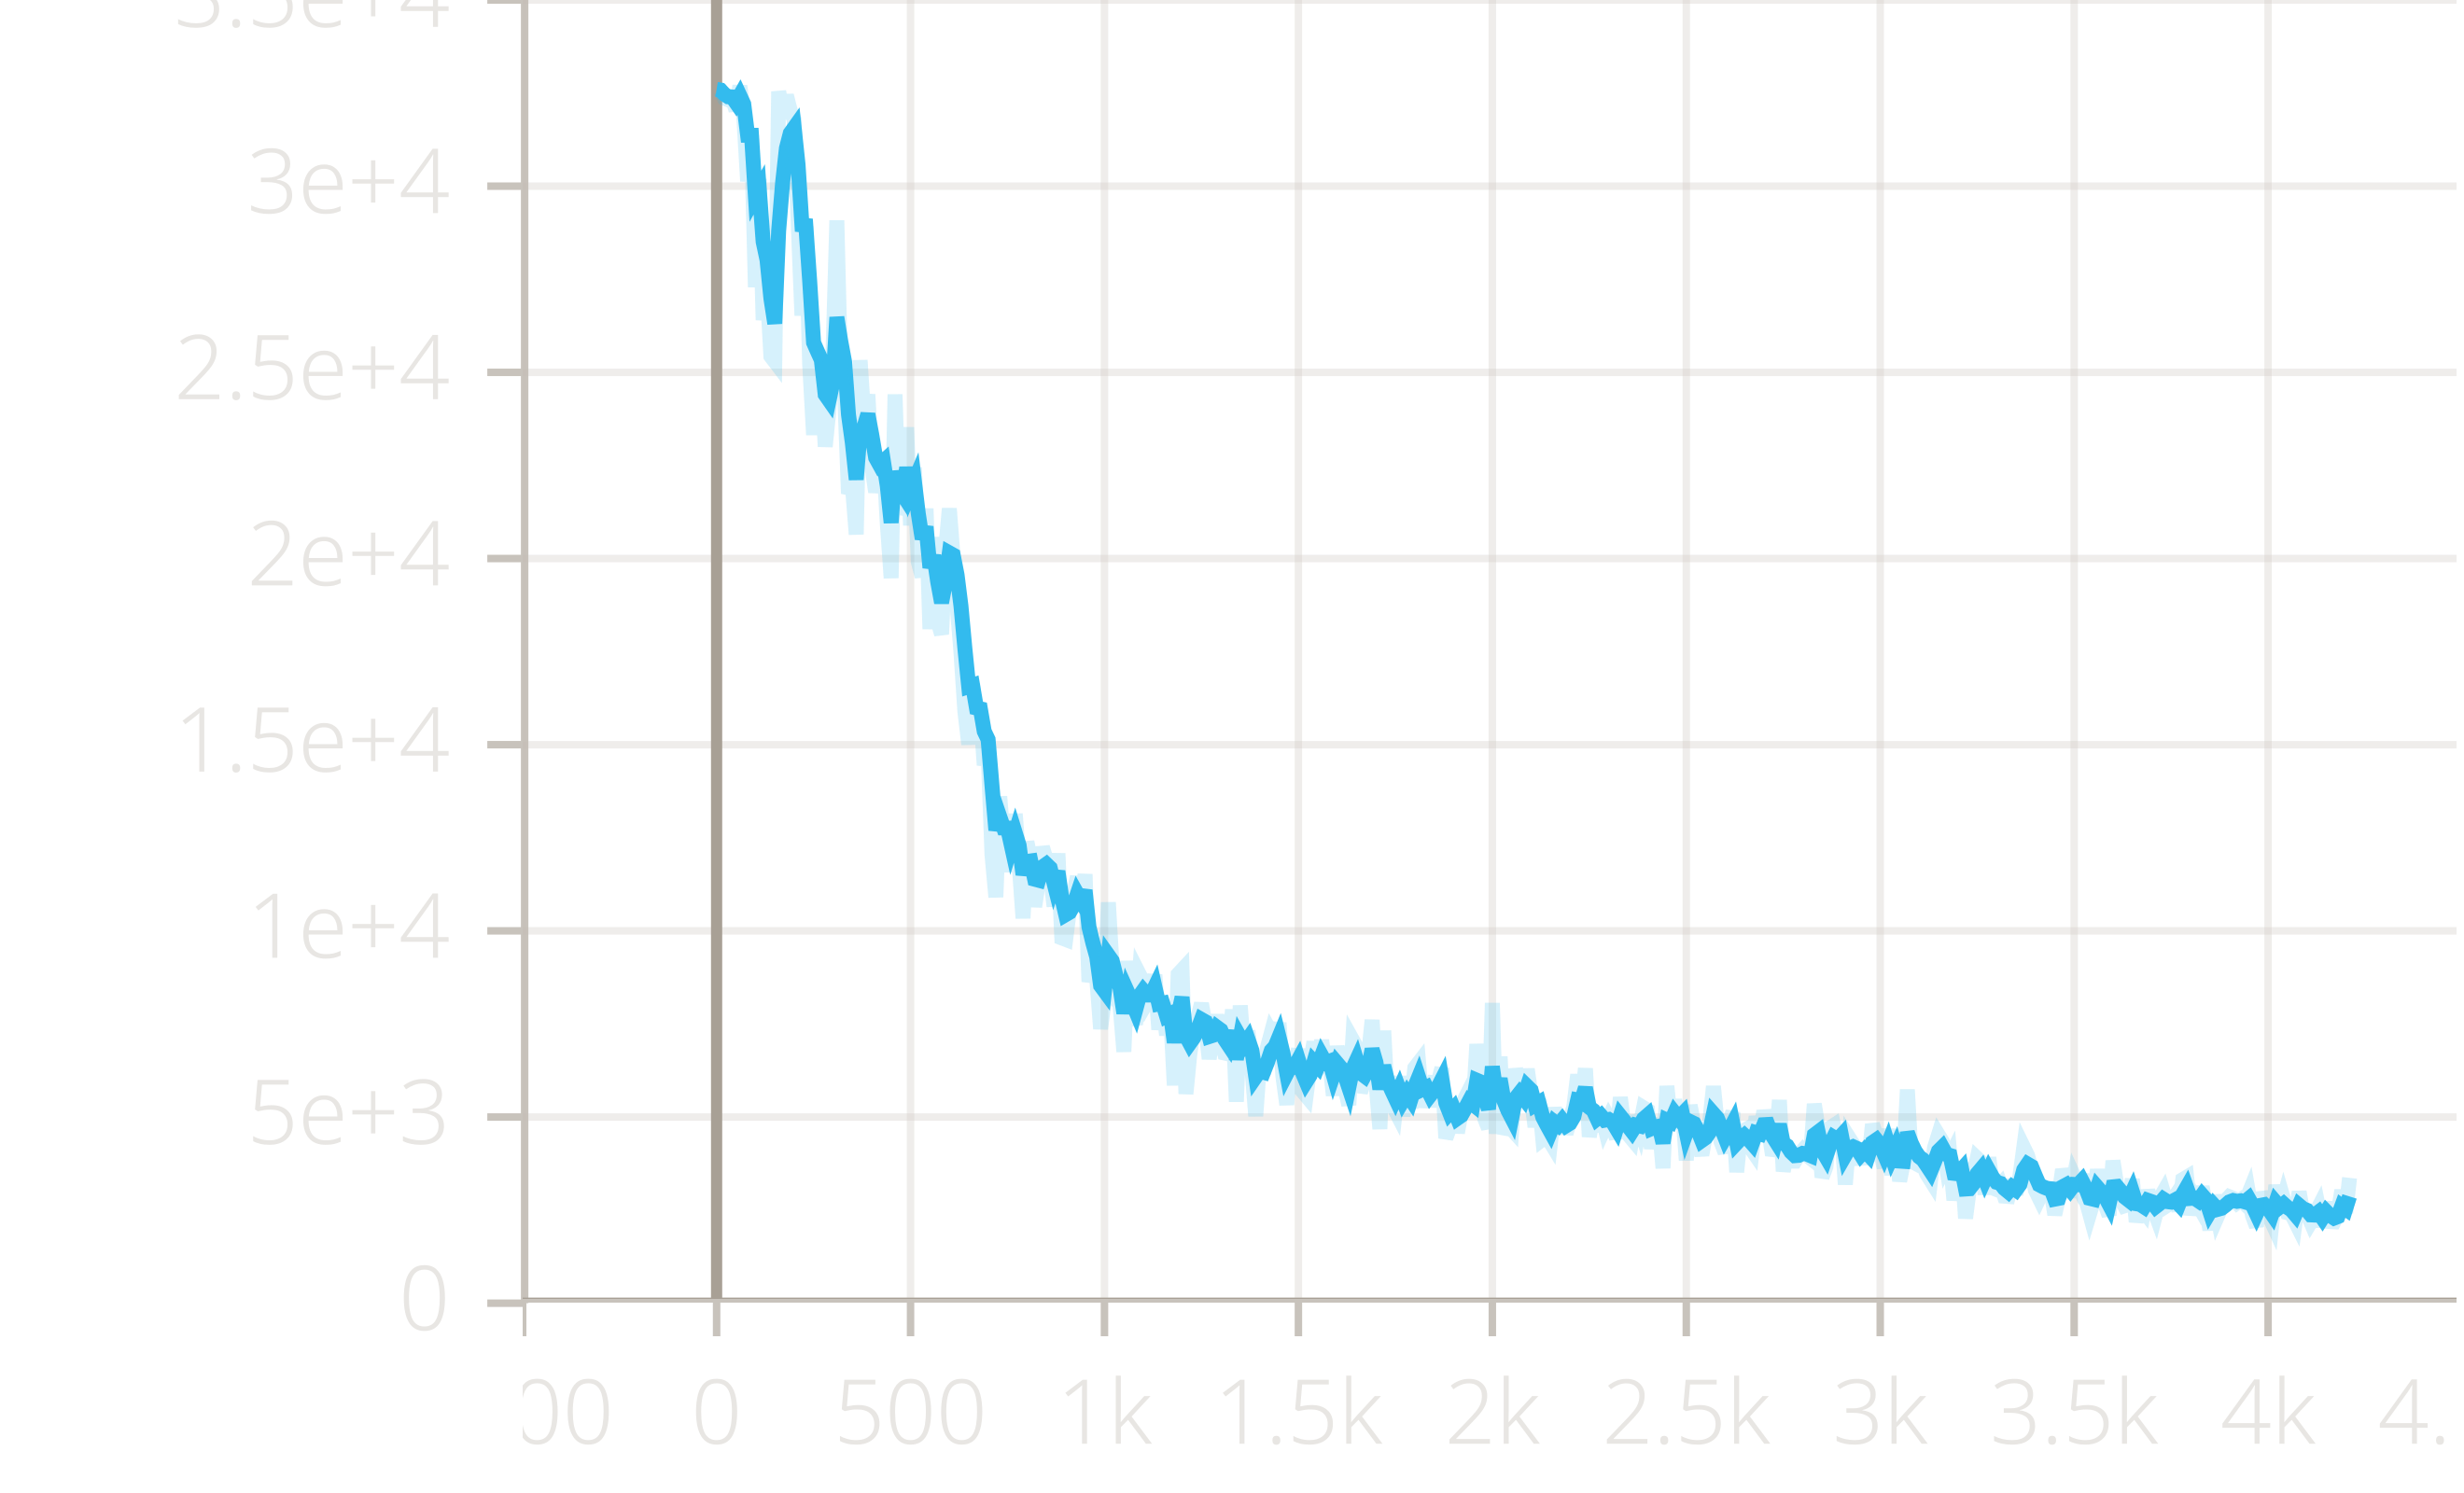
\includegraphics[width=\textwidth]{figures/loss_train.png}
        \caption{开发集上的loss}
    \end{minipage}
    \begin{minipage}[H]{0.5\linewidth}
        \centering
        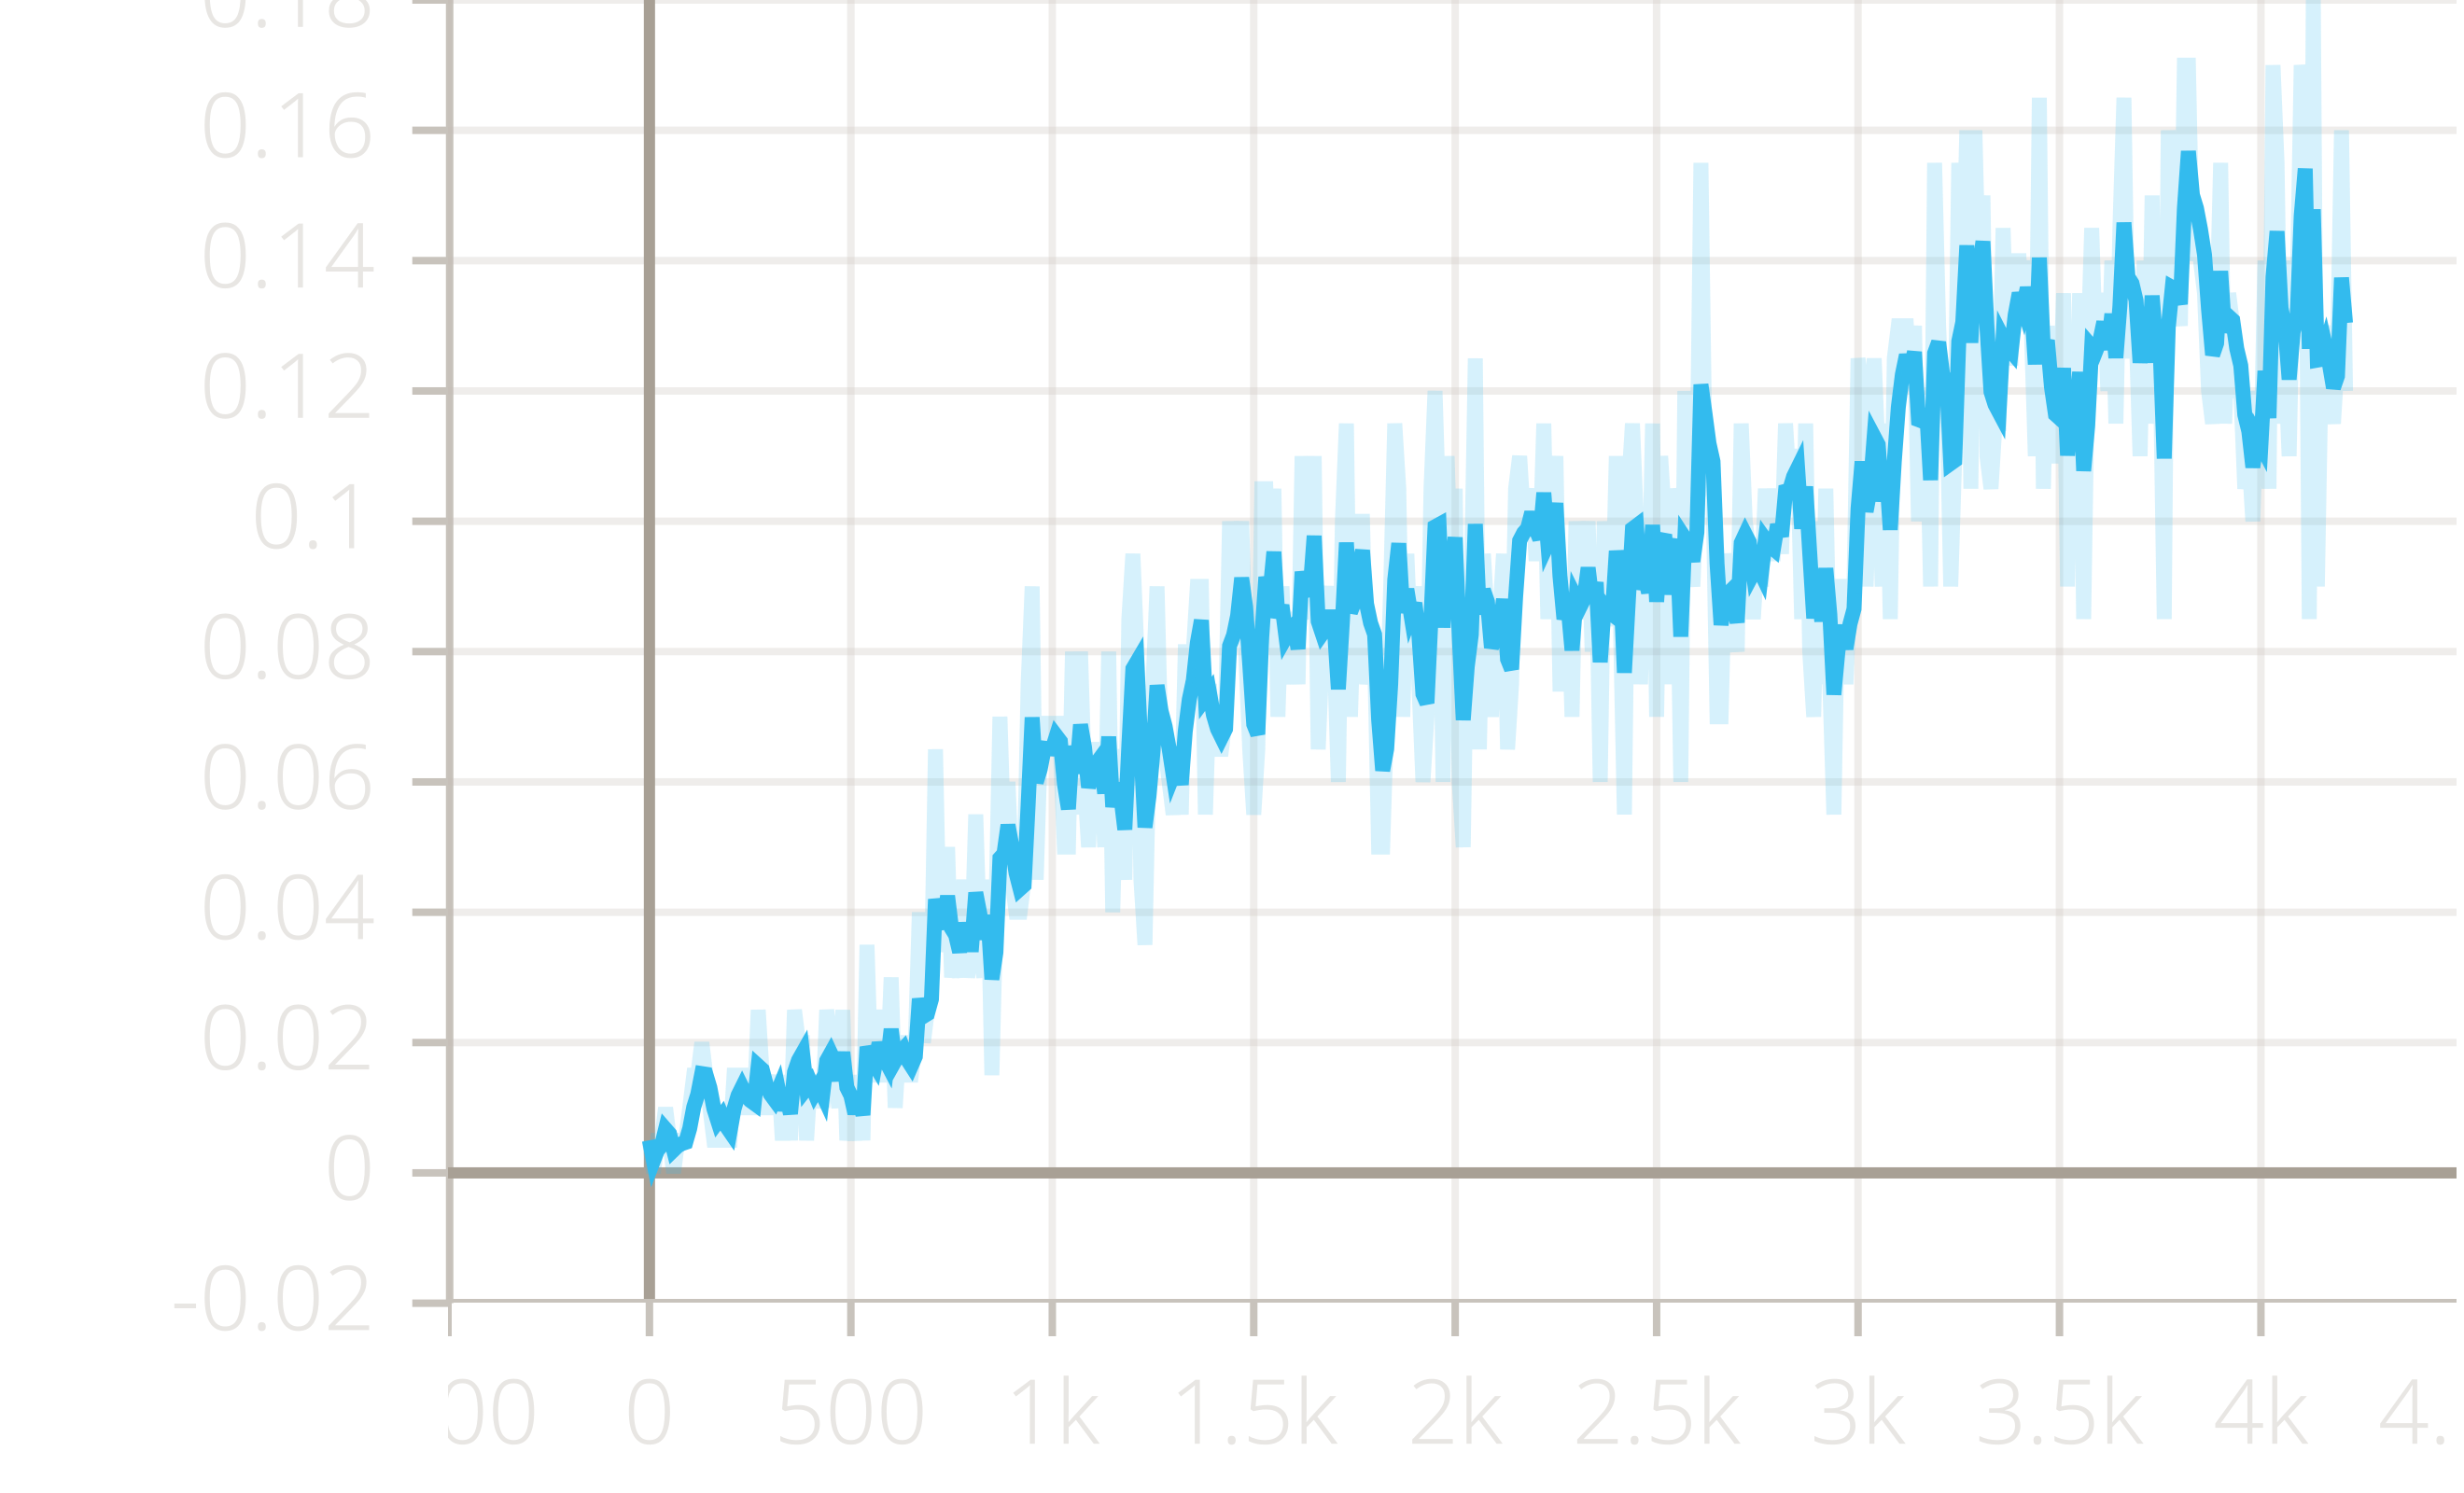
\includegraphics[width=\textwidth]{figures/acc_dev.png}
        \caption{开发集上的acc}
    \end{minipage}
    \label{dev}
\end{figure}

可见LSTM对说话人的鉴别能力有一定效果。

\bibliographystyle{unsrt}
\bibliography{refs}

\end{document}
